%% Measurement Science and Technology (IOP Publishing) submission.
%% Prepared with the official IOP template iopjournal.cls, downloaded 2026-09-15
%% from https://publishingsupport.iopscience.iop.org/wp-content/uploads/2025/07/ioplatextemplate.zip
%%
%% TO COMPILE: keep iopjournal.cls, orcid.pdf and fig1.pdf .. fig4.pdf in this
%% same directory (IOP requires a flat directory, no subfolders), then run
%% pdflatex twice.
%%
%% ARTICLE TYPE: Paper (full research paper, not a Technical Design Note,
%% which IOP caps at about 2500 words).
%%
%% All fields are filled; there are no remaining placeholders. Verified with
%% src/check_mst_compliance.py and src/audit_submission.py, which also compiles
%% this file and re-derives every quoted number from the sealed result files.

\documentclass{iopjournal}

\usepackage{amsmath,amssymb}
\usepackage{graphicx}
\usepackage{booktabs}
\usepackage{url}

\begin{document}

\articletype{Paper}

\title{Allocating camera views and time instants for trajectory-length
measurement under a frame-processing budget}

\author{Bowen Tan$^1$\orcid{0009-0007-0554-9261},
Zihan Li$^3$,
Shengjie Guo$^4$\orcid{0009-0004-6852-4836},
Yi Sui$^2$\orcid{0009-0001-8081-5183},
Xiaolei Zhang$^2$\orcid{0000-0002-0122-4554},
Yi Li$^2$\orcid{0000-0002-4185-3152}
and Jun Ji$^{2,*}$\orcid{0000-0003-3194-2183}}

\affil{$^1$The Hong Kong University of Science and Technology, Clear Water Bay,
Kowloon, Hong Kong SAR, China}

\affil{$^2$College of Computer Science and Technology, Qingdao University,
308 Ningxia Road, Qingdao 266071, China}

\affil{$^3$College of Mathematics and Statistics, Qingdao University,
308 Ningxia Road, Qingdao 266071, China}

\affil{$^4$Inner Mongolia Agricultural University, 306 Zhaowuda Road,
Saihan District, Hohhot 010018, Inner Mongolia, China}

\affil{$^*$Author to whom any correspondence should be addressed.}

\email{junji@qdu.edu.cn}

\keywords{vision-based measurement, distance travelled, trajectory length,
multi-camera triangulation, sampling design, measurement uncertainty,
budget allocation}

\begin{abstract}
A multi-camera trajectory-length measurement can divide a finite processing
budget between simultaneous views and sampling instants. We evaluate this
allocation using released image centroids from a seven-camera rig and an
independent optical tracking reference. Original protocol-frozen results are
distinguished from exploratory analyses on four previously examined records.
A calibration-selected three-view configuration at 28 instants gives a mean
absolute error of 9.60 mm, compared with 50.77 mm for seven views at 12
instants, at exactly 84 processed frames per window. This ordering persists
under three observation-noise settings, reference decimation and deletion of
each record in turn. However, a broader grid of budget caps and two to seven
views reveals a reversal: at 168 frames, the tested three-view schedule has
85.66 mm error versus 10.55 mm for seven views, driven by rare extreme errors.
Thus spending an increased budget on more instants can worsen performance,
and no universal three-view prescription follows. Comparisons report actual
frame use, completed-window error, completion and tail risk. Overlapping-camera
noise controls constrain possible explanations without identifying a causal
saturation mechanism. A tested curvature-based sampling rule is evaluated on
explicit common-success populations, and a secondary single-camera case
illustrates an aggregate sparse-sampling preference with incomplete primary
confirmation. The study provides a reproducible evaluation procedure for
budget-dependent measurement choices, with explicit reference sensitivity
and limits on generalization.

\end{abstract}

% =====================================================================
\section{Introduction}
\label{sec:introduction}

A recurring measurement task is to report how far a target moved over a time
window: the arc length of its trajectory, rather than the straight-line
displacement between the endpoints. When the trajectory is observed only at
discrete instants, the estimate is biased in two directions at once.
Connecting sparse samples by straight lines cuts every corner and
underestimates the arc. With non-vanishing independent position noise, dense sampling can accumulate
noise-driven length, and the limiting polyline length can diverge. This
conclusion is conditional on the noise model; a constant position offset
does not change length.

This trade-off is established. Palmer [1] simulated it for fishing-vessel
tracks and noted that the overestimation at high polling rates is inversely
proportional to vessel speed. Ranacher \textit{et al} gave a closed form for
the noise-driven overestimate [2] and devoted a separate study to locating the
balance point for floating-car data [3]. Noonan \textit{et al} [4] established
the full picture for animal telemetry, proved the divergence result, named the
balance point the `Goldilocks sampling frequency', argued that it is
impractical to hit deliberately, and published a corrective estimator.
Rowcliffe \textit{et al} [5] and Schoombie \textit{et al} [6] quantified the
two limbs empirically. We claim none of this as new and we build on it
directly.

It is also known that adding cameras to a markerless motion-capture rig helps
less than one might expect. Mulla \textit{et al} [7] found that two cameras
can match four for markerless hand tracking, and Walker \textit{et al} [8]
found that eighteen, twelve and six cameras change biomechanical kinematics by
only a few degrees. We report the existence of saturation as confirmation of
their finding, not as a discovery.

What neither literature contains is the allocation question that these two
facts jointly create. A telemetry collar has one sensor and a fixed duty
cycle, so the sampling interval is its only lever, and the practical response
to the bias trade-off is post-hoc correction. A camera rig has two levers, and
they compete for the same budget. If the cost that matters is the number of
camera frames that must be transferred, decoded, detected and triangulated,
then a budget of $B$ frame reads per window satisfies
\begin{equation}
B = k\,m,
\label{eq:budget}
\end{equation}
where $k$ is the number of simultaneous views used at each instant and $m$ is
the number of instants. The design question is where to spend. The saturation
studies [7, 8] vary the camera count at a fixed frame rate, and so measure
only one edge of that surface.

This paper contributes the following.

\begin{enumerate}
\item \textit{An explicit frame-budget comparison.} The camera count and
sampling density are varied jointly. At an equal budget of 84 frames, the
calibration-selected triple at 28 instants has a confirmation-set error of
9.60\,mm against 50.77\,mm for seven views at 12 instants. This comparison is
an exploratory analysis of configurations recorded under the frozen protocol.
A broader budget-cap grid includes two through seven views and exposes
budget-dependent rank reversals and rare large errors.

\item \textit{Controls on a possible explanation.} We compare an
independent-pixel-noise geometry model with observed reconstruction errors,
disjoint camera groups, a shared-camera noise simulation and a robust
triangulation baseline. The results distinguish evidence for correlated
errors from a causal or quantitative decomposition of their sources.

\item \textit{Tests of further tuning and its costs.} We quantify the
performance of one curvature-based placement rule, including an oracle-assisted
version, without claiming a general optimum. We also separate typical errors
from rare extreme errors and report the completion loss of robustness gates.

\end{enumerate}

We follow the vision-based measurement framing of Shirmohammadi and Ferrero
[9]: the camera rig is the instrument, and the object of study is the
measurand and its uncertainty, not the performance of an algorithm.
Section~\ref{sec:opposite} provides a contrasting case study of a
single-camera chained-registration system, where the smallest tested budget
has the lowest aggregate error, with incomplete primary confirmation. This is why
we present allocation as a quantity to evaluate per instrument.

% =====================================================================
\section{Related work}
\label{sec:related}

\subsection{Sampling-density bias in distance travelled}
The two-sided bias, the interior optimum, and its dependence on the ratio of
motion per interval to measurement noise are established in [1--4]. Noonan
\textit{et al} [4] give a practical sampling window bounded below by the ratio
of error variance to velocity variance and above by the velocity
autocorrelation time, prove that no estimator recovers distance when the
sampling interval exceeds three times that autocorrelation time, and provide a
continuous-time speed and distance estimator. Codling and Hill [10] give
analytic expressions for how apparent step length scales with sampling rate in
a correlated random walk; Jerde and Visscher [11] and Hurford [12] document
the noise-driven corruption of step lengths and turn angles. The fractal and
tortuosity literature [13, 14] is the conceptual antecedent. All of this work
treats a single sensor with a fixed sampling rate.

\subsection{Camera count in multi-view measurement}
Triangulation uncertainty as a function of camera count, baseline and noise is
characterised in [15], and diminishing returns are expected. Markerless
motion-capture studies report saturation empirically [7, 8, 16]. Leizea
\textit{et al} [17] build an uncertainty budget for a multi-camera system and
test the premise that more viewpoints lower uncertainty. These analyses hold
the temporal sampling fixed and vary only the view count, so they do not
address a shared budget.

\subsection{Network design and negative results in measurement}
Shen \textit{et al} [18] derive network-configuration guidance from an error
characterisation of an industrial photogrammetric system, which is the closest
methodological precedent to what we do, but for a static network and a static
measurand. Nasiri \textit{et al} [19] show that a textbook optimal
triangulation method is not optimal, and Das \textit{et al} [20] show that a
widely used agreement statistic misrepresents markerless versus marker-based
comparison; our sections~\ref{sec:nonuniform} and \ref{sec:outliers} are of
that kind.

\subsection{Positioning}
Our contribution is the budget axis of equation~\eqref{eq:budget}, empirical
allocation comparisons, and controls on possible explanations and tuning. The bias mechanism
belongs to [1--4]; the existence of saturation belongs to [7, 8].

% =====================================================================
\section{Measurand, measurement chain and cost model}
\label{sec:chain}

\subsection{Measurand}
The arc length of the target's trajectory between two specified instants, in
metres. We report it separately from the endpoint displacement, which is a
different quantity and behaves differently under sampling.

\subsection{Chain}
At each selected instant the target's image position in each selected camera
is triangulated by the direct linear transform into a three-dimensional point.
The sequence of positions is converted to a length by one of three estimators:

\begin{itemize}
\item \textit{Polygon}: the sum of the segment lengths.
\item \textit{Limited arc}: a segment-wise Hermite interpolation with a
limiter that removes backward longitudinal overshoot while retaining
transverse curvature, integrated by 32-point Gauss--Legendre quadrature.
\item \textit{State mean}: the length of the conditional mean path of a
Wiener-velocity state-space model fitted to the selected positions, with the
acceleration spectral density chosen by innovation likelihood [21]. This is
the strongest of the three at realistic budgets and is the primary estimator
throughout. Unless stated otherwise, the isotropic observation standard
deviation is 3\,mm. The acceleration spectral density is selected from 13
log-spaced values between $10^{-6}$ and $10^{3}$\,m$^{2}$\,s$^{-3}$ by
innovation likelihood, and speed is integrated with eight quadrature points
per interval. These settings are held fixed across view counts.
\end{itemize}

A fourth estimator integrates the conditional expected speed. By Fubini's
theorem the integral of the expected speed equals the expectation of the
integrated speed, so this implements the conditional-expectation principle of [4] under our
Wiener-velocity model. It is not a reproduction of their fitted stochastic
model or model-selection procedure; section~\ref{sec:ctsd} evaluates this
model-specific baseline with calibrated observation noise.

\subsection{Cost model}
One camera frame read at one instant is one unit, so a window costs $B=k\,m$.
Frames in which the detector returns nothing are still charged. It is a proxy for processing load, not a measured runtime or energy cost:
transfer, decoding, detection and triangulation need not have equal or linear
costs across implementations. Calibration is treated as a fixed setup cost.
The budget deliberately does not count acquisition: a rig that records seven cameras and processes three has
already paid for the sensors. The model therefore answers how much of a
recorded multi-camera stream must be processed, not how many cameras to buy.

\subsection{Error dispersion and reference sensitivity}
\label{sec:uncertainty}
For the calibration-selected triple at $m=33$, 60 confirmation windows have
a mean reference length of 6.625\,m. Table~\ref{tab:uncertainty} reports a
conditional, top-down error summary. The signed bias is $-8.23$\,mm and the
standard deviation of signed errors is 7.43\,mm. No bias correction is
applied to any reported estimate. A correction of $+8.23$\,mm estimated on
these same windows would centre their errors by construction; its transfer
to new records and its estimation uncertainty have not been validated.

\begin{table}
\caption{Conditional error summary for the selected triple at 33 instants
(99 frames per window). Dispersion and reference sensitivity are reported
separately; no combined uncertainty or coverage interval is asserted.}
\centering
\begin{tabular}{llr}
\hline
Quantity & Evaluation & Value (mm)\\
\hline
Signed bias, $b$ & uncorrected & $-8.23$\\
Error dispersion, $s_e$ & window standard deviation & $7.43$\\
Reference sensitivity scale, $s_r$ & decimation proxy & $0.55$\\
\hline
\end{tabular}
\label{tab:uncertainty}
\end{table}

The reference sensitivity proxy is the mean range of reference polyline
lengths at strides one, two and four, divided by $\sqrt{3}$. Treating this
range as a rectangular half-width is only a sensitivity convention; it does
not characterize optical-reference calibration, scale or synchronization
uncertainty. Reference errors may already contribute to $s_e$, so these
quantities are not combined in quadrature. Section~\ref{sec:saturation}
instead evaluates the principal comparison directly under reference decimation.

The 60 windows share four records, one rig and one calibration session.
Consequently, 59 independent degrees of freedom and 95\% coverage cannot be
asserted. Common calibration, reference-system and timing errors may not be
represented by between-window variation. A complete instrument uncertainty
assessment would require those contributions, their covariance, independent
calibration information and coverage validation on additional sessions.
Section~\ref{sec:saturation} instead reports paired record-level sensitivity
intervals for comparisons, and section~\ref{sec:mechanism} examines temporal
error structure without treating it as a full uncertainty propagation model.

\subsection{Failure policy}
An instant at which fewer than two views yield a detection is dropped from the
polyline. If either endpoint instant is lost, the window is a failure.
Failures remain in completion-rate denominators. Error summaries use
completed windows; paired comparisons use the intersection of completed
windows and report its size. A failed window has no finite error assigned.
The earlier non-uniform sampling experiment used stricter, sequential
eligibility screens; its distinct policy and conditional sample sizes are
specified in section~\ref{sec:nonuniform}.

% =====================================================================
\section{Data and frozen protocols}
\label{sec:data}

\subsection{Primary rig}
Seven hardware-synchronised cameras at 50\,Hz observe a single passive marker
carried through free-space motion, and an optical tracking system records the
marker at 200\,Hz as an independent reference [22]. We use the publisher's
released per-camera two-dimensional centroids and intrinsics, with extrinsics
fitted once on the separate calibration record 3. Each record gives 15 non-overlapping windows
of 3.98\,s, that is 200 camera frames. Development used records 19 to 23,
giving 75 windows. Confirmation used records 15 to 18, giving 60 windows,
previously touched only by a per-frame triangulation quality check and never
by any path, sampling or estimator design.

\subsection{Secondary chain, opposite regime}
Three sequences from a public colour-and-depth benchmark [23] with a single
moving camera and an optical tracking reference for the camera pose. Positions
come from chained pairwise rigid registrations, not independent triangulation.
Development used the 15 windows at offsets 1 to 17\,s used by earlier work;
confirmation used the 14 valid windows at offsets of at least 21\,s, never
previously touched.

\subsection{Protocol freezing and analysis status}
For each confirmation run the protocol, candidate list, camera-subset rule,
decision gates and source-file hashes were frozen before the path-length
confirmation predictions were computed. Predictions were sealed by a
cryptographic hash before the reference was loaded for that run's scoring.
The primary rig's confirmation records had already been used for per-frame
triangulation quality checks, as noted above; they were not wholly unseen
data. The released local timestamps and hashes document this execution
sequence, rather than an independently timestamped public preregistration.

On the primary rig, the frozen candidates compared a 57-frame selected
triple and a 56-frame pair against a 56-frame seven-view baseline; the
one-frame mismatch is retained explicitly. Same-density comparisons and the
84-frame comparison use the recorded secondary grid. The record-resampling
intervals, disjoint-group and noise controls, and robust-triangulation
comparison reported here are exploratory analyses made after confirmation
outcomes were examined. No equivalence margin was specified in advance.
The additional budget-cap grid uses $B\in\{56,84,112,168\}$ and
$k=2,\ldots,7$, with uniform $m=\lfloor B/k\rfloor$ instants. The existing
calibration-only subset score is extended to four, five and six views before
computing this grid, without optimizing subsets on reference errors. Noise
sensitivity at $B=84$ uses fixed $\sigma=0.4,1,3$\,mm, spanning the earlier
development-derived scale and the original setting. These choices were made
after inspecting earlier results and remain exploratory; they are neither a
new holdout nor a fresh preregistration. Of the recalculated estimates, 288
overlap the archived primary-rig estimates and reproduce them exactly.
For the secondary chain, XFeat was the pre-specified primary front end and
ORB was secondary; both results are reported in section~\ref{sec:opposite}.

\subsection{Reference caveat}
The reference length is the polyline of the 200\,Hz trace between the window
endpoints, itself a sampled estimate. Decimating it by two changes the
reference length by a few millimetres, the scale of the smallest differences
we report.

% =====================================================================
\section{Results}
\label{sec:results}

\begin{figure}
\centering
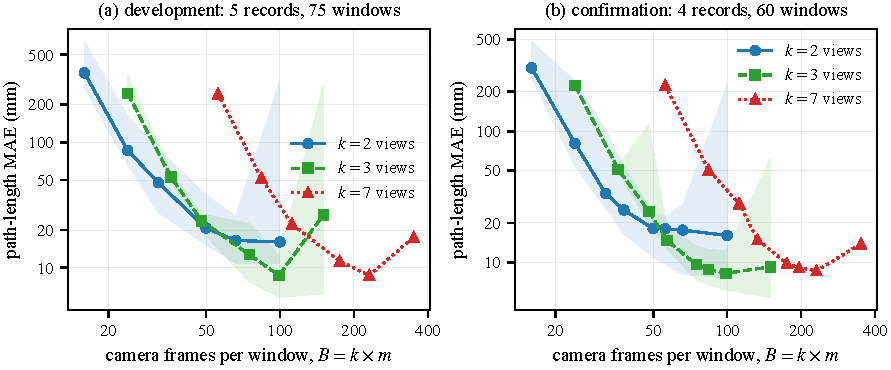
\includegraphics[width=\textwidth]{fig1.pdf}
\caption{Exploratory budget-cap grid using one calibration-selected subset
per view count and $m=\lfloor B/k\rfloor$ uniform instants. (a) Completed-window
MAE; pairs complete 48/60 windows and the other view counts complete 60/60.
(b) The 95th percentile and maximum error for three and seven views. These
are tested schedules using nearly all the cap, not a lower error envelope
over all schedules costing at most $B$.}
\label{fig:frontier}
\end{figure}

\subsection{Trading view count for sampling density}
\label{sec:saturation}
Figure~\ref{fig:frontier} shows the new budget-cap grid. Before describing
it, we distinguish original frozen decisions and same-density summaries.
Figure~\ref{fig:saturation} and table~\ref{tab:confirm} summarize all subsets
at fixed density on the protocol-frozen confirmation set.

\begin{table}
\caption{Original frozen candidate comparisons against the seven-view,
eight-instant baseline (56 frames, 223.42\,mm MAE, 60/60 complete). Each
candidate had to reduce MAE by at least 50\%, improve every record and incur
no additional failures. The protocol explicitly allowed 56/57 frames. MAE
is conditional on each arm's completed windows.}
\centering
\begin{tabular}{rrrrrl}
\hline
Views & Instants & Frames & MAE (mm) & Complete & Decision\\
\hline
2 & 28 & 56 & 12.52 & 48/60 & Fail: completion\\
3 & 19 & 57 & 14.86 & 60/60 & Pass\\
\hline
\end{tabular}
\label{tab:originaldecisions}
\end{table}

Table~\ref{tab:originaldecisions} reports the original decisions, not the
new exploratory grid. The triple passed all stated gates but spent one
extra frame; this is not an exactly equal-cost result. The pair's completed
MAE is not a like-for-like comparison to all 60 baseline windows: the
baseline MAE on its 48 common windows is 270.88\,mm. Its completion gate
nevertheless failed. The separate 66-frame pair was not a primary candidate.

\begin{figure}
\centering
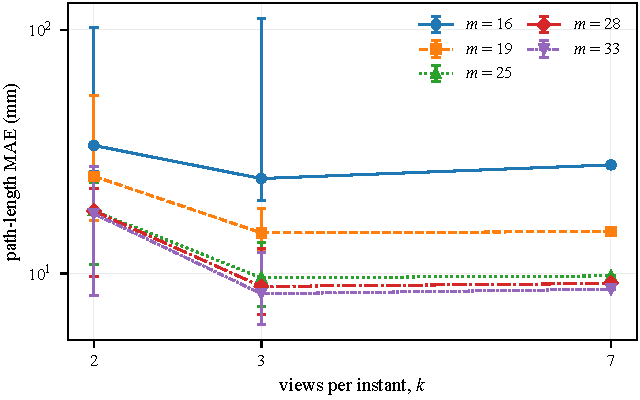
\includegraphics{fig2.pdf}
\caption{Error against the number of views at fixed sampling density on the
protocol-frozen confirmation set. The bars span the best to the worst camera subset of that size; they are
not confidence intervals. Subset medians are descriptive summaries, not the
performance of the pre-selected triple.}
\label{fig:saturation}
\end{figure}

\begin{table}
\caption{Confirmation set, 60 windows, state-mean estimator. Median over
camera subsets of the mean absolute error, in millimetres, and the number of
failed window-arms.}
\centering
\begin{tabular}{rrrrl}
\hline
$m$ & $k=2$ & $k=3$ & $k=7$ & failed, $k=2/3/7$\\
\hline
16 & 33.6 & 24.5 & 27.9 & 250 / 0 / 0\\
19 & 25.1 & \textbf{14.7} & 14.9 & 250 / 0 / 0\\
25 & 18.1 & \textbf{9.6} & 9.8 & 250 / 0 / 0\\
28 & 18.1 & \textbf{8.8} & 9.1 & 250 / 0 / 0\\
33 & 17.6 & \textbf{8.3} & 8.6 & 250 / 0 / 0\\
\hline
\end{tabular}
\label{tab:confirm}
\end{table}

The subset medians in table~\ref{tab:confirm} are close for three and seven
views at $m\geq19$, but they do not identify a deployable subset and the 35
triples are not independent replicates. We therefore report the single triple
selected by the frozen calibration-only rule separately. Its camera IDs are
216f21c1, 3e0f8f0 and 44c4b2e; the rule minimizes the worst-pair geometric
error scale at a calibration-derived scene centre.

\begin{table}
\caption{Exploratory comparison of the pre-selected triple with all seven
views on 60 completed confirmation windows. Differences are three-view minus
seven-view MAE. Intervals resample the four whole records with replacement
(all $4^4$ combinations), retaining their 15 windows each. Four clusters give
limited inferential resolution; these are not equivalence tests.}
\centering
\begin{tabular}{rrrrl}
\hline
$m$ & Triple MAE & Seven-view MAE & Difference & 95\% resampling interval (mm)\\
\hline
16 & 72.79 & 27.92 & $+44.87$ & $[-0.27,134.93]$\\
19 & 14.86 & 14.87 & $-0.01$ & $[-0.41,0.29]$\\
25 & 10.08 & 9.79 & $+0.29$ & $[-0.37,0.70]$\\
28 & 9.60 & 9.12 & $+0.48$ & $[0.10,0.82]$\\
33 & 9.25 & 8.63 & $+0.62$ & $[0.19,0.93]$\\
\hline
\end{tabular}
\label{tab:recordpairs}
\end{table}

At $m=33$, record-specific differences are $+0.67$, $+1.01$, $-0.02$ and
$+0.82$\,mm for records 15--18. Thus the selected triple is slightly worse
in aggregate, despite using 99 instead of 231 frames (43\%). A nonsignificant
difference at some other settings would not establish equal accuracy either.
At $m=16$, one dropout leaves the selected triple with two views and produces
a 3.1\,m error, giving a mean of 72.79\,mm rather than the 24.5\,mm median
over all triples. Completion alone therefore does not establish reliability.
Across the 21 pairs, 250 of 1260 window-arms fail at each listed density,
against zero of 2100 for the triples.

At an exactly equal cost of 84 frames, the selected triple at 28 instants
gives 9.60\,mm versus 50.77\,mm for seven views at 12 instants, with all
60 windows completed. Every record favours the triple, with MAE differences
between $-46.21$ and $-36.03$\,mm; the exploratory record-resampling interval
is $[-45.08,-37.25]$\,mm. This supports allocating more instants on this
rig within the tested grid, not a universal optimal view count. Separately,
three views at 19 instants cost 57 frames and give 14.86\,mm, versus
27.92\,mm at 112 frames for seven views at 16 instants: a lower-cost,
lower-error comparison, not an equal-cost comparison.


\subsubsection{Budget-cap and parameter sensitivity.}
Table~\ref{tab:budgetcaps} broadens the analysis to two through seven views.
All configurations use the same 60 windows and original 3\,mm noise setting.
Pairs complete only 48 windows, so their MAE cannot alone rank them above
complete configurations. Within configurations completing all windows, the
lowest observed MAE is at four views for $B=56$, three for $B=84$ and 112,
and six for $B=168$. These are post-hoc rankings, not validated selection rules.

\begin{table}
\caption{Exploratory budget-cap grid: MAE in millimetres, with actual processed
frames in parentheses. Each view count uses one calibration-only subset.
Pairs complete 48/60 windows in every row; all other configurations complete
60/60. Full per-record, percentile and maximum errors are supplied in the archive.}
\centering
\small
\begin{tabular}{rrrrrrr}
\hline
Cap $B$ & 2 views & 3 views & 4 views & 5 views & 6 views & 7 views\\
\hline
56 & 12.52 (56) & 71.07 (54) & 36.08 (56) & 84.35 (55) & 139.13 (54) & 223.42 (56)\\
84 & 10.79 (84) & 9.60 (84) & 77.24 (84) & 40.00 (80) & 33.92 (84) & 50.77 (84)\\
112 & 9.83 (112) & 8.88 (111) & 10.78 (112) & 18.66 (110) & 29.01 (108) & 27.92 (112)\\
168 & 9.61 (168) & 85.66 (168) & 25.45 (168) & 9.13 (165) & 8.61 (168) & 10.55 (168)\\
\hline
\end{tabular}
\label{tab:budgetcaps}
\end{table}

At 168 frames the triple encounters two errors above 100\,mm, with a maximum
of 4110.45\,mm, whereas the seven-view maximum is 24.92\,mm. At the 56-frame
cap, one triple error reaches 3233.05\,mm. Completion therefore does not
guarantee reliability, and using more of an available budget need not help.
An upper budget permits retaining a cheaper schedule: the 84-frame triple
is still feasible at a cap of 168. The table evaluates specified near-cap
schedules, not the optimum over every allocation with $km\leq B$.

At 84 frames, the three/seven-view MAEs are 8.36/49.97\,mm for
$\sigma=0.4$\,mm, 8.48/50.04\,mm for 1\,mm and 9.60/50.77\,mm for
3\,mm, with 60/60 completions throughout. Thus this particular ordering is
stable over the tested settings. These are shared isotropic-noise sensitivity
settings, not individually optimized covariance models or a test of every
weighted reconstruction.

For the original 3\,mm setting at 84 frames, the four record differences are
all negative; deleting one whole record gives differences from $-42.88$ to
$-39.49$\,mm. At 112 frames, the deletion range is $[-21.67,-12.62]$\,mm,
while at 168 frames it is $[10.14,101.23]$\,mm: the adverse ranking remains
after deleting any one record. These descriptive checks do not turn four
records into a larger independent sample. Resampling intervals above retain
their exploratory interpretation.

Keeping each reference window's endpoints and decimating only its interior
200\,Hz samples at strides one, two and four changes the 84-frame MAE
difference from $-41.17$ to $-41.14$ and $-41.07$\,mm. Its ordering also
persists at the two alternative noise settings. This directly tests
reference-resolution sensitivity of the main contrast; it does not test
reference calibration, clock offset or absolute scale errors.

\subsection{Error structure and controls on the saturation hypothesis}
\label{sec:mechanism}
Saturation at a handful of cameras has been reported before [7, 8].
Table~\ref{tab:mechanism} summarizes position-error diagnostics on the five
development records; the controls below examine possible explanations without
identifying a unique mechanism.

\begin{table}
\caption{Predicted and realised effect of using seven views instead of three,
on the five development records. The independent-pixel-noise model predicts a
ratio near 0.59; the realised ratio averages 1.08. The median cosine is taken
between the three-view and seven-view position error vectors.}
\centering
\begin{tabular}{lrrrrrl}
\hline
Record & 3 views & 7 views & Realised & Model & Median & Best six-view\\
 & RMS (mm) & RMS (mm) & ratio & ratio & cosine & subset\\
\hline
19 & 3.078 & 2.369 & 0.770 & 0.589 & 0.881 & drop cam.\ 1: 2.274 ($-4.0$\%)\\
20 & 3.146 & 2.412 & 0.767 & 0.586 & 0.875 & drop cam.\ 1: 2.323 ($-3.7$\%)\\
21 & 2.992 & 4.415 & \textbf{1.476} & 0.593 & 0.869 & drop cam.\ 6: 2.437 ($-44.8$\%)\\
22 & 17.047 & 7.765 & 0.456 & 0.583 & 0.866 & drop cam.\ 2: 6.411 ($-17.4$\%)\\
23 & 2.958 & 5.678 & \textbf{1.920} & 0.591 & 0.868 & drop cam.\ 2: 3.179 ($-44.0$\%)\\
\hline
\end{tabular}
\label{tab:mechanism}
\end{table}

\subsubsection{The geometric prediction.}
Under independent isotropic pixel noise the triangulation covariance is
\begin{equation}
\mathrm{Cov}(\mathbf{X}) = \sigma_{\mathrm{px}}^{2}
\left( \sum_{i=1}^{k} \mathbf{J}_{i}^{\top}\mathbf{J}_{i} \right)^{-1},
\label{eq:cov}
\end{equation}
where $\mathbf{J}_{i}$ is the $2\times3$ projection Jacobian of camera $i$ at
the point $\mathbf{X}$. Evaluated along the reference trajectory, this model
predicts a seven-view to three-view error ratio of 0.583 to 0.593 across the
five records, that is, seven views should be about 41\% more accurate.

\subsubsection{The realised ratio.}
The realised ratio averages 1.08, and on two records the seven-view solution
is worse than the three-view one.

\subsubsection{Correlated errors and overlapping subsets.}
The median cosine between three-view and seven-view error vectors is 0.866
to 0.881. This measures directional agreement, not the fraction of shared
error variance. The reconstructions reuse three cameras and the same
reference, so correlation alone cannot identify calibration or centroid bias.

An exploratory linearized least-squares simulation uses the projection
Jacobians along every fortieth development reference point, 100 independent
unit-variance Gaussian pixel-noise draws per point, and shared noise draws
for cameras present in both solutions. Even with an exact reference and
independent noise across cameras, the nested three/seven-view median cosine
is 0.738--0.753 across records. The observed nested cosine therefore cannot
be interpreted without this overlap control.

The selected three cameras and the remaining four form disjoint groups.
Their observed error cosine is 0.418--0.459, compared with 0.004--0.008 in
the independent-noise simulation. This is consistent with shared error
sources, but common reference error and model mismatch remain alternatives;
we do not identify a causal contribution or a shared-variance percentage.

\subsubsection{Temporal structure and path-length sensitivity.}
For a polygon with segment unit directions $\mathbf{u}_i$ and position
errors $\mathbf{e}_i$, the first-order length perturbation is
\begin{equation}
\delta L \approx \sum_i \mathbf{u}_i^{\mathrm T}
                         (\mathbf{e}_{i+1}-\mathbf{e}_i).
\label{eq:pathperturbation}
\end{equation}
A constant translation cancels, whereas a shared but time-varying error need
not. The ratio of adjacent error-increment RMS to position-error RMS for the
selected triple is 0.31, 0.33, 0.37, 1.39 and 0.32 on records 19--23,
respectively. Four records show temporal persistence, while record 22
contains strong increments. These position-level diagnostics do not propagate
uncertainty through the nonlinear state-mean estimator or prove why its
length errors saturate.

\subsubsection{Sensitivity to reconstruction robustness.}
Removing the best single camera retrospectively reduces seven-view position
RMS on each development record by 3.7\% to 44.8\%. This oracle removal
diagnostic does not define a prospective selection rule. We additionally
apply an existing pixel-consensus triangulation rule at seven views and
33 instants, using a fixed 4-pixel threshold and majority support of at least
four views, without temporal gating. On the same 75 development windows,
state-mean path MAE is 8.697\,mm with consensus, 8.699\,mm with seven-view
DLT and 8.809\,mm with the selected three-view DLT. All 75 windows complete;
one of 2475 queried instants is rejected by consensus. Thus this control
changes path error little at this density. It does not establish that all
robust or weighted reconstructions behave similarly, or that additional
views are intrinsically harmful. The measured allocation surface remains
conditional on the calibration, estimator and detection regime.

\subsection{A curvature-based non-uniform sampling rule}
\label{sec:nonuniform}
For a smooth curve the deficit of one segment is approximately
\begin{equation}
\Delta_{i} \approx \frac{(\Delta t_{i})^{3}}{24}\,
\kappa_{i}^{2}\,\lVert \mathbf{v}_{i} \rVert^{3},
\label{eq:deficit}
\end{equation}
with $\kappa$ the curvature and $\mathbf{v}$ the velocity. Write
$a(t)=\kappa(t)^2\lVert\mathbf{v}(t)\rVert^3$ and let $n(t)$ be the number
of intervals per unit time. In the small-interval approximation, the total
polygon deficit is $\int_0^T a(t)/(24n(t)^2)\,dt$, subject to
$\int_0^T n(t)\,dt=m-1$. Variation with a Lagrange multiplier gives
$-a/(12n^3)+\lambda=0$, hence $n(t)\propto a(t)^{1/3}$. This continuous
density problem, rather than minimization of a fixed-coefficient discrete
sum over interval lengths, gives the rule

\begin{equation}
\rho(t) = \left(\kappa^{2}\lVert\mathbf{v}\rVert^{3}\right)^{1/3}
= \frac{\lVert \mathbf{v}\times\mathbf{a}\rVert^{2/3}}
{\lVert \mathbf{v}\rVert}.
\label{eq:rho}
\end{equation}
Unlike a telemetry collar, a camera system can actually execute such a
placement, so this is the natural next lever after the budget split.

We tested three arms at identical cost: uniform placement; a deployable arm
that spends half the budget on a uniform probe, fits the state model, computes
$\rho$ from the smoothed trajectory and places the remaining instants at equal
increments of the cumulative $\rho$ while keeping the probe instants; and an
oracle arm that computes $\rho$ from the reference trajectory. The oracle uses otherwise unavailable trajectory information to evaluate
this particular rule. It is neither deployable nor a certified optimum for
path-error minimization, even within curvature-driven methods. Figure~\ref{fig:nonuniform} and
table~\ref{tab:nonuniform} give the result.

\begin{figure}
\centering
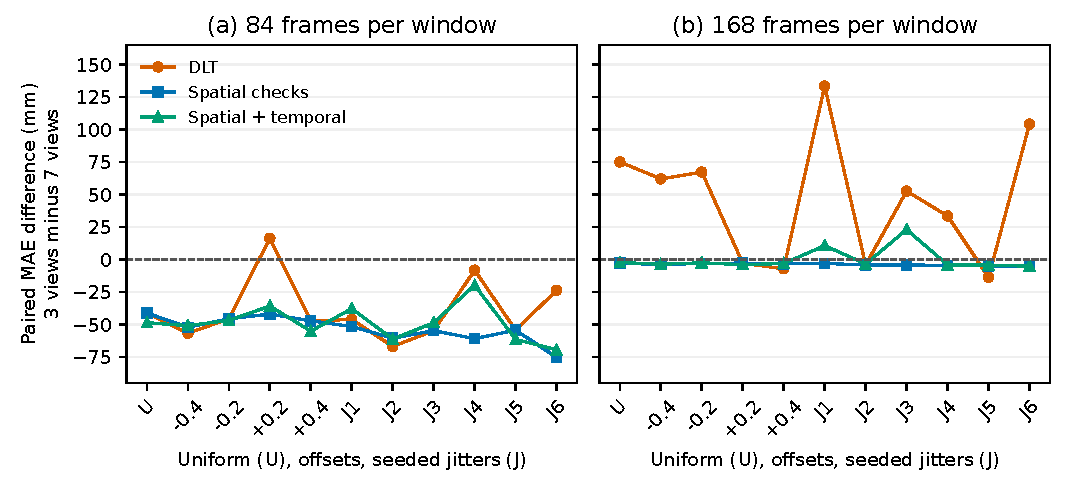
\includegraphics{fig3.pdf}
\caption{Non-uniform placement of instants on the development set, at three
views. The reference-assisted rule improves completed-window MAE by approximately
7.9\% to 23.5\% in the plotted three-view cells. The deployable rule is worse
on their respective common-success populations.}
\label{fig:nonuniform}
\end{figure}

\begin{table}
\caption{Non-uniform placement on a pool of 75 development windows.
State-mean MAEs (mm) use only the common-success windows in the last-column
denominator. The numerator counts windows where the deployable rule beats
uniform placement. Eligibility and successful-output counts are given below.}
\centering
\begin{tabular}{rrrrrl}
\hline
$k$ & $m$ & Uniform & Curvature & Oracle & Deployable wins\\
\hline
3 & 8  & 270.7 & 458.0 & 223.2 & 12 / 67\\
3 & 16 & 20.7  & 54.3  & 16.7  & 7 / 63\\
3 & 25 & 9.2   & 15.9  & 8.4   & 10 / 61\\
3 & 33 & 7.6   & 10.1  & 7.0   & 18 / 62\\
7 & 8  & 242.9 & 425.5 & 200.9 & 13 / 75\\
7 & 33 & 7.4   & 9.8   & 6.6   & 20 / 75\\
\hline
\end{tabular}
\label{tab:nonuniform}
\end{table}

The recorded successful outputs for uniform/deployable/reference-assisted
arms, respectively, are 71/69/67, 66/64/64, 67/62/63 and 66/63/62 out of
75 for the listed three-view densities; all three arms have 75 outputs in
the listed seven-view cells. The common sets contain 67, 63, 61 and 62 windows.
Unlike the main experiment, this earlier implementation requires every
selected instant to be valid and screens uniform, probe and later stages
sequentially. Some absent downstream outputs were never attempted, so these
counts are not independent per-method completion probabilities. The comparisons
are conditional on joint eligibility, not a claim about overall operational
success. The additional noise-calibration burst is a setup resource excluded
from the within-window frame count.

The deployable rule has higher aggregate MAE in every tested cell, by
30\% to 170\%. Two possible explanations, not isolated by ablation, are that equation~\eqref{eq:deficit} holds only for small $\Delta t$, so
concentrating instants in high-curvature regions creates long gaps whose cubic
penalty may outweigh local gains; and curvature estimated from a
half-budget probe may be noisy.

Reference-assisted curvature placement improves on uniform sampling by
8\% to 25\%, with a median of 17\% across the tested cells. This describes
one rule and one grid. The small-interval polygon approximation does not
optimize the final state-mean estimator's absolute error. An earlier
reference-based enumeration gave about 35\% improvement by selecting instants
against the final error directly. The gap cannot be assigned quantitatively
to error cancellation or to recoverable signal from these experiments.
Neither experiment bounds what another adaptive or learned rule could gain.

\subsection{A calibrated continuous-time estimator does not remove the effect}
\label{sec:ctsd}
A natural objection is that the corrective estimator of [4] should be used
instead of characterising the allocation. We evaluate its conditional-expected-speed principle
within our state model, rather than reproduce the full method. We calibrated the
observation noise from a dense consecutive burst at the native frame interval,
assuming that measurement noise dominates process noise, obtaining 0.20 to 0.43\,mm
per record and subset.

Calibrating the noise gives a small consistent improvement to the state-mean
estimator, from 8.81 to 7.86\,mm at three views and 33 instants. The
conditional-speed estimator does reduce sensitivity to sampling density at the
sparse end, as designed: at seven views and eight instants it gives 165.2\,mm
against 242.9\,mm. But it carries a large positive bias at every setting
tested, $+42$ to $+180$\,mm, and is dominated in absolute error by the
conditional-mean-path estimator throughout. We attribute this to model
misspecification rather than to the method: [4] uses an
Ornstein--Uhlenbeck process with a fitted velocity autocorrelation time and
selects the model by a corrected information criterion, whereas our
Wiener-velocity model has none. We therefore do not claim that the method of
[4] fails, only that with our state model it does not remove the allocation
effect in this implementation. This comparison does not rule out a
better-specified stochastic model. The dense probe used for noise calibration
is an additional calibration resource, outside the per-window frame budget.

\subsection{Rare extreme errors dominate the dense-regime mean}
\label{sec:outliers}
The mean absolute error over our windows rises at high sampling density, which
invites the interpretation that the classical noise-inflation limb has been
reached. The distribution, in table~\ref{tab:outliers} and
figure~\ref{fig:regimes}(a), shows the importance of rare extreme errors.

\begin{table}
\caption{Development set at three views, state-mean estimator with calibrated
noise, in millimetres, as a function of the number of instants. The median broadly falls then stabilizes, increasing slightly from
5.8 to 6.1\,mm at the final setting; the ninetieth percentile falls. The
mean rises mainly because of one window at 50 instants and one at 200.}
\centering
\begin{tabular}{lrrrrrrr}
\hline
Statistic & 8 & 16 & 25 & 33 & 50 & 100 & 200\\
\hline
Mean & 269.6 & 21.1 & 10.0 & 7.9 & \textbf{29.4} & 6.5 & \textbf{35.2}\\
Median & 114.0 & 16.8 & 8.8 & 6.6 & 6.1 & 5.8 & 6.1\\
90th percentile & 592.8 & 41.7 & 20.6 & 15.7 & 13.5 & 12.6 & 11.5\\
Maximum & 1893.7 & 60.6 & 29.2 & 26.8 & \textbf{1691.6} & 20.3 & \textbf{2182.5}\\
Windows over 100\,mm & 38 & 0 & 0 & 0 & \textbf{1} & 0 & \textbf{1}\\
\hline
\end{tabular}
\label{tab:outliers}
\end{table}

The rise in the mean at 50 and at 200 instants is produced by a single window
each, in which one instant received a grossly wrong triangulation. This is
outlier exposure: denser sampling draws more instants and has more
opportunities to include a bad one. An order-of-magnitude estimate of the
classical mechanism for this rig, with calibrated white noise near 0.4\,mm and
about 34\,mm of motion per 20\,ms step, gives roughly 2\,mm of inflation at
the densest setting, consistent with the median flattening near 5 to 6\,mm
rather than rising.

These observations motivate robustness checks without excluding simultaneous
noise accumulation. A combined view-consensus and Kalman-innovation gate
reduces the median completed-window MAE across 35 triples from 38\,mm to
6\,mm at 200 instants and improves 34 triples. It rejects inconsistent
observations, and rejects a window if an endpoint is lost. Only 2432 of
2625 window-arms complete (92.6\%), compared with 2625 without the gate;
193 failures accompany the error reduction. The error summaries therefore
condition on different completed populations and do not isolate the effect
of temporal gating. The same gate hurts some lower-density settings by
rejecting real motion. A deployment decision must assess completion and error
together. Mean error alone cannot distinguish smooth noise accumulation from
rare gross failures.

\subsection{The opposite regime: chained single-camera egomotion}
\label{sec:opposite}
In the secondary chain the positions come from chained pairwise rigid
registrations of a single moving camera. Each edge contributes registration
noise that does not shrink with more edges, while the roughly 0.8\,m of smooth
motion in a 4\,s window is nearly fully captured by eight instants.
Figure~\ref{fig:regimes}(b) and table~\ref{tab:opposite} give the result on 14
unseen windows.

\begin{figure}
\centering
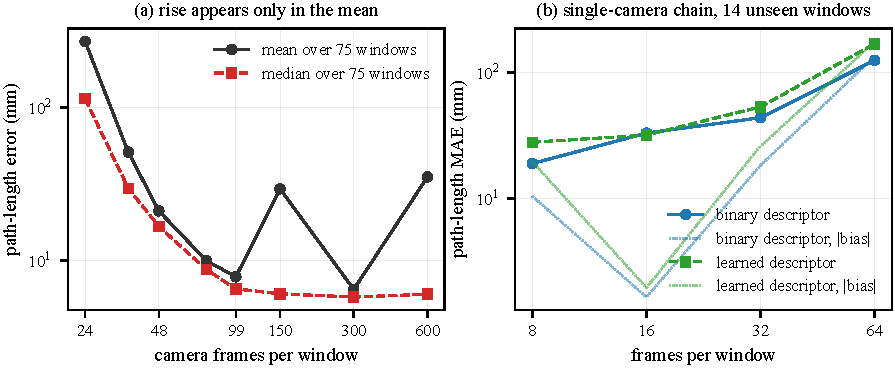
\includegraphics[width=\textwidth]{fig4.pdf}
\caption{(a) Rare extreme errors dominate the dense-regime rise in the mean;
the median remains near 6\,mm.
(b) The tested single-camera chain favours fewer frames in aggregate, and
the magnitude of the signed bias reaches a minimum between 16 and 32 frames,
where the bias changes sign.}
\label{fig:regimes}
\end{figure}

\begin{table}
\caption{Secondary chain, 14 confirmation windows. MAE in millimetres with
signed bias in parentheses; both are averaged within each sequence and then
equally across the three sequences (2, 7 and 5 windows). XFeat is primary;
ORB is secondary.}
\centering
\begin{tabular}{lrrrr}
\hline
Front end & 8 frames & 16 & 32 & 64\\
\hline
ORB (secondary) & \textbf{18.9} ($-10.0$) & 33.0 ($-6.9$) & 43.8 ($+11.4$) & 125.6 ($+91.1$)\\
XFeat (primary) & \textbf{27.9} ($-18.3$) & 31.8 ($-2.2$) & 53.5 ($+26.0$) & 170.0 ($+146.8$)\\
\hline
\end{tabular}
\label{tab:opposite}
\end{table}

The frozen primary criterion required XFeat's sequence-equal MAE at eight
frames to beat both 32 and 64 frames overall, not exceed the 32-frame error
in any sequence, and complete at least as many windows as at 32 frames.
It was not fully met: the aggregate and completion conditions passed, but
the per-sequence condition failed. ORB passed the same criteria as a
pre-specified secondary analysis. Both front ends completed all 14 windows
at every budget. Thus the aggregate trends and the secondary result support
a sparse-sampling preference in this chain, but the primary confirmation
does not establish it across all sequences. The signed bias changes sign
between 16 and 32 frames, consistent with competing sampling and registration
effects. Fourteen windows from three sequences on the same rig do not
establish transfer to other instruments.

% =====================================================================

\section{Limitations}
\label{sec:limitations}
\begin{itemize}
\item \textit{Two instruments, each a single rig.} The budget-cap grid has different best observed view counts and rank
reversals. No universal three-view optimum or saturation threshold is established.
The controls in section~\ref{sec:mechanism} do not identify a unique
causal mechanism; calibration, reference error, estimator choice and target
visibility can all affect the observed surface.
\item \textit{Published detections, not raw pixels.} For the multi-camera rig
we use the publisher's released centroids, so detection cost and detection
failure modes are inherited rather than measured.
\item \textit{The cost model counts processing, not acquisition.} A
capture-design reading, namely to buy three cameras rather than seven, is not
supported, because a rig built with three cameras would have different
occlusion behaviour.
\item \textit{Reference resolution.} Differences of one to three millimetres
are within the sensitivity of the reference polyline to its own sampling.
\item \textit{One target, free-space motion.} No occlusion-heavy, multi-target
or articulated cases are covered.
\item \textit{One sampling rule.} The reference-assisted rule in
section~\ref{sec:nonuniform} is not an upper bound on other curvature-based,
adaptive or learned schedules.
\item \textit{Limited confirmation.} The record-level analyses have only four
clusters, and the primary single-camera criterion was not fully met. The
additional sensitivity analyses are exploratory, not fresh confirmations.
\end{itemize}

% =====================================================================
\section{Conclusion}
\label{sec:conclusion}
For this synchronised rig, allocating 84 frames to three views at 28
instants gives lower observed MAE than seven views at 12 instants, and this
contrast persists under the tested noise settings, reference decimation and
whole-record deletion. The broader two-to-seven-view budget grid nevertheless
reverses the three/seven-view ranking at 168 frames because of rare large
errors. Thus a budget increase is not a prescription to sample more densely,
and the lowest-error tested schedule is not a universal camera-count rule.
At a fixed 33 instants the selected triple uses 43\% of the frames but has
slightly larger error; equivalence remains unestablished.

The reusable procedure is to specify a processing cap and failure policy,
select camera subsets without using evaluation errors, and compare feasible
schedules using error, completion, tail risk and sensitivity together. A
prospective deployment would require selection on development data followed
by validation on new records or sessions; the new grid here is exploratory.
Correlated-error diagnostics do not identify a unique mechanism, and the
curvature-rule comparisons condition on explicit joint eligibility. The
single-camera example illustrates a contrasting regime with incomplete
primary confirmation. These qualifications delimit the measurement choices
supported by the present evidence.

% =====================================================================

% Back matter. iopjournal.cls generates the headings automatically.
% =====================================================================

\ack{The authors used a large language model based artificial intelligence
assistant (OpenAI GPT) under author direction to help implement the
analysis scripts, to run the experiments reported here, to build the tooling
that re-derives every number in this manuscript from the sealed result files,
and to draft and revise the text. The manuscript distinguishes protocol-frozen
confirmation runs from exploratory analyses. Reported numbers were checked
against the archived results and derived analysis files, and the
authors take full responsibility for the content of the publication.

The authors declare no conflict of interest: no employment, consultancy, stock
ownership, honoraria, paid expert testimony, patent application or other
financial or personal relationship has influenced the work reported here.}

\funding{This research did not receive any specific grant from funding
agencies in the public, commercial or not-for-profit sectors.}

% Contributor roles use the NISO CRediT taxonomy, https://credit.niso.org
\roles{\textbf{Jun Ji:} data curation, methodology, formal analysis,
resources, writing -- original draft.
\textbf{Zihan Li:} software, formal analysis, writing -- review and editing.
\textbf{Bowen Tan:} software, formal analysis, writing -- review and editing.
\textbf{Shengjie Guo:} supervision, validation, writing -- review and editing.
\textbf{Yi Sui:} software, formal analysis, validation, writing --
review and editing.
\textbf{Xiaolei Zhang:} supervision, project administration, writing --
review and editing.
\textbf{Yi Li:} supervision, project administration, writing -- review and
editing.}

\data{The two datasets analysed here are third-party public releases, cited as
[22] and [23]; we redistribute neither, and the access routes are those given
by their publishers. The analysis code, frozen protocols, input hash lists, sealed
predictions, scoring records and revised manuscript are archived as version 1.0.3
at \url{https://doi.org/10.5281/zenodo.22794671}. The matching source release is
\url{https://github.com/Jun-Jason-Ji/views-or-instants/tree/v1.0.3}.
The version preserves the original protocols and sealed results, alongside
the exploratory analysis update with explicit sequence-equal aggregation,
record-level comparisons and exploratory geometry controls, with input hashes
and a reproducible analysis script. Protocol freezing and prior data exposure
are described in section~\ref{sec:data}.}

% =====================================================================
% thebibliography prints its own "References" heading; a \section* here
% would print it twice.
\begin{thebibliography}{99}

\bibitem{palmer2008} Palmer M C 2008 Calculation of distance traveled by fishing vessels
using GPS positional data: a theoretical evaluation of the sources of error
\textit{Fish. Res.} \textbf{89} 57--64

\bibitem{ranacher2016a} Ranacher P, Brunauer R, Trutschnig W, Van der Spek S and Reich S
2016 Why GPS makes distances bigger than they are
\textit{Int. J. Geogr. Inf. Sci.} \textbf{30} 316--33

\bibitem{ranacher2016b} Ranacher P, Brunauer R, Van der Spek S and Reich S 2016 What is an
appropriate temporal sampling rate to record floating car data with a GPS?
\textit{ISPRS Int. J. Geo-Inf.} \textbf{5} 1

\bibitem{noonan2019} Noonan M J \textit{et al} 2019 Scale-insensitive estimation of
speed and distance traveled from animal tracking data
\textit{Mov. Ecol.} \textbf{7} 35

\bibitem{rowcliffe2012} Rowcliffe J M, Carbone C, Kays R, Kranstauber B and Jansen P A 2012
Bias in estimating animal travel distance: the effect of sampling frequency
\textit{Methods Ecol. Evol.} \textbf{3} 653--62

\bibitem{schoombie2024} Schoombie S, Wilson R P, Ropert-Coudert Y, Dilley B J and Ryan P G
2024 The efficiency of detecting seabird behaviour from movement patterns: the
effect of sampling frequency on inferring movement metrics in
Procellariiformes \textit{Mov. Ecol.} \textbf{12} 59

\bibitem{mulla2025} Mulla D M, Majoni N, Tilley P M and Keir P J 2025 Two cameras can
be as good as four for markerless hand tracking during simple finger movements
\textit{J. Biomech.} \textbf{181} 112534

\bibitem{walker2026} Walker R, Robinson M A, Outerleys J \textit{et al} 2026 The effect
of camera configuration on multi-camera markerless motion capture for
biomechanical analysis \textit{J. Biomech.} \textbf{206} 113522

\bibitem{shirmohammadi2014} Shirmohammadi S and Ferrero A 2014 Camera as the instrument: the
rising trend of vision based measurement
\textit{IEEE Instrum. Meas. Mag.} \textbf{17} 41--47

\bibitem{codling2005} Codling E A and Hill N A 2005 Sampling rate effects on measurements
of correlated and biased random walks
\textit{J. Theor. Biol.} \textbf{233} 573--88

\bibitem{jerde2005} Jerde C L and Visscher D R 2005 GPS measurement error influences on
movement model parameterization \textit{Ecol. Appl.} \textbf{15} 806--10

\bibitem{hurford2009} Hurford A 2009 GPS measurement error gives rise to spurious
180-degree turning angles and strong directional biases in animal movement
data \textit{PLoS ONE} \textbf{4} e5632

\bibitem{turchin1996} Turchin P 1996 Fractal analyses of animal movement: a critique
\textit{Ecology} \textbf{77} 2086--90

\bibitem{benhamou2004} Benhamou S 2004 How to reliably estimate the tortuosity of an
animal's path \textit{J. Theor. Biol.} \textbf{229} 209--20

\bibitem{lee2020} Lee S H and Civera J 2020 Robust uncertainty-aware multiview
triangulation \textit{arXiv} 2008.01258

\bibitem{nakano2020} Nakano N \textit{et al} 2020 Evaluation of 3D markerless motion
capture accuracy using OpenPose with multiple video cameras
\textit{Front. Sports Act. Living} \textbf{2} 50

\bibitem{leizea2023} Leizea I, Herrera I and Puerto P 2023 Calibration procedure of a
multi-camera system: process uncertainty budget
\textit{Sensors} \textbf{23} 589

\bibitem{shen2023} Shen X, Yue J, Dou S and Huang G 2023 Network configuration and
repeatability precision of industrial photogrammetry
\textit{Measurement} \textbf{211} 112589

\bibitem{nasiri2023} Nasiri S-M, Hosseini R and Moradi H 2023 The optimal triangulation
method is not really optimal \textit{IET Image Process.} \textbf{17} 2855--65

\bibitem{das2023} Das K, de Paula Oliveira T and Newell J 2023 Comparison of
markerless and marker-based motion capture systems using 95\% functional
limits of agreement \textit{Sci. Rep.} \textbf{13} 22880

\bibitem{sarkka2023} S\"arkk\"a S and Svensson L 2023 \textit{Bayesian Filtering and
Smoothing} 2nd edn (Cambridge: Cambridge University Press)

\bibitem{primaryrig} Jatesiktat P, Lim G M and Ang W T 2024 Multi-camera
calibration using far-range dual-LED wand and near-range chessboard fused in
bundle adjustment \textit{Sensors} \textbf{24} 7416; MCalib dataset available
at \url{https://koonyook.github.io/MCalib/}

\bibitem{sturm2012} Sturm J, Engelhard N, Endres F, Burgard W and Cremers D 2012 A
benchmark for the evaluation of RGB-D SLAM systems \textit{Proc. IEEE/RSJ Int.
Conf. on Intelligent Robots and Systems} pp 573--80

\end{thebibliography}

\end{document}
